\section{Controller}

Snake is only fun if you can actually control the snake. The STK500 have 8 switches which could have been used, but they are both hard to press precisely and fast. They are also clunky as you would have to either hold the whole board or lean over it. To combat this we added a old NES Controller from the Nintendo Entertainment System. It's a simple controller, also with 8 buttons. It uses a TC4021B 8-Stage Static Shift Register and uses its parellel in / serial out operations to transfer which buttons are pushed.

\subsection{NES Controller}

We are using the NES Controller in our project and need to write a driver to interface with the chip in that controller.
The chip in the controller are a TC4021B, and we have used to datasheet\cite{toshiba:tc4021b} to figure out how to interface with it.

The TC4021B has five connections available to us:
\begin{itemize}
\item Ground
\item Clock
\item Latch
\item Data
\item Vcc
\end{itemize}

Instead of cutting the cord on the controller, we bought an extension coord, we have therefor mapped the colours of the signals in the extension coord below.

\begin{figure}
\centering
\begin{BVerbatim}
         +----> Vcc    (yellow)
         |
4 +---------+ 6
 | x  x  o   \
 | o  o  o  o |
3 +-----------+ 0
   |  |  |  |
   |  |  |  +-> Ground (brown)
   |  |  +----> Pulse  (orange)
   |  +-------> Latch  (black)
   +----------> Data   (red)
\end{BVerbatim}
\caption{NES Controller extension cord}
\label{fig:nes}
\end{figure}

Mapping of the signals in the NES extention coord.

We need all the pins connected for the controller to work. The Vcc needs to be 5 V as 3 V is not enough to drive the TC4021B.

As we interface with the serial part of the TC4021B we use the Latch to shift between parallel mode and serial mode, the Clock to pulse the bits out, and the Data to read the bits.

The controller can be in 2 modes: Parallel and Serial.

Parallel mode is When the Latch is high, the controller is in parellel mode and the buttons state is continuously "latched" into the TC4021B. The data pin will also be set to the first bit's state.

Serial mode is when the Latch is low. In this state the Data pin has the state of the "current bit" and each time you make a pulse on the Clock pin the bit's are shifted. Therefore you need 7 pulses to read 8 bits out. After the 7 pulses the Latch needs to be set to high again, to get the new inputs as seen in Figure~\ref{fig:controller_cycle}

\begin{figure}
\centering
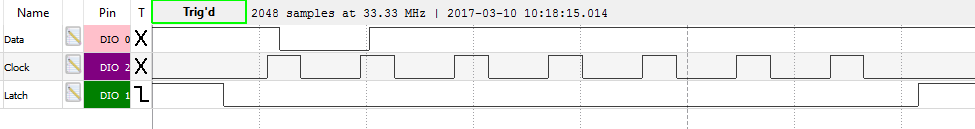
\includegraphics[width=0.8\textwidth]{architecture/controller_cycle}
\caption{A full transmission, where the B buttons is pushed}
\label{fig:controller_cycle}
\end{figure}

The order of the states of the buttons are transfered are found by simply trial, as there is no official public datasheet for the controller. The order are as follows A, B, Select, Start, Up, Down, Left, Right.

\subsection{SPI driver}

As we use the hardware SPI interface for the screen, we choose to implement the controller with a software SPI driver. It uses a few template inputs.

\begin{itemize}
\item SPI Pin Collection ( The 3 pins needed to use SPI )
\item Number of Bits that needs transfered ( The controller needs 8 )
\item 4 Delay timers ( Descriped more in the implementation )
\end{itemize}
